
\documentclass[11pt]{article}
\usepackage{amsmath, amssymb}
\usepackage{geometry}
\usepackage{hyperref}
\usepackage{graphicx}
\usepackage{booktabs}
\geometry{margin=2.5cm}

\newcommand{\ket}[1]{|#1\rangle}
\newcommand{\bra}[1]{\langle#1|}
\newcommand{\Oedge}{X_0 Z_1\cdots Z_{L-2} X_{L-1}}

\title{Week 6 Notes: From One Measurement to a Phase Diagram}
\author{Seminar notes}
\date{\today}

\begin{document}
\maketitle

\section{Purpose of Week 6}

Week 5 established a proof of principle: after mapping the Kitaev chain to qubits, a gate-prepared state can reveal topology through a non-local Pauli string. The Week 5 example was deliberately narrow. It focused on the topological sweet spot
\begin{equation}
  t=\Delta, \qquad \mu=0,
\end{equation}
and measured the boundary string
\begin{equation}
  X_0 Z_1 Z_2 X_3
\end{equation}
for a four-site chain.

Week 6 turns this single-point demonstration into a phase diagnostic. The parameter $\mu$ is swept through trivial, critical, and topological regimes. The central question is:
\begin{quote}
  Can the same circuit-measurable non-local string reconstruct the known phase boundary $|\mu|=2t$?
\end{quote}

This is still part of Block 3, not yet the full Block 4 noise study. The role of Week 6 is to define the ideal observable curve that later noisy-circuit simulations should be compared against.
\section{From Week 5 to Week 6: What Changes Conceptually}

Week 5 established that topology can be detected after Jordan--Wigner mapping using a non-local Pauli string evaluated on a single fine-tuned point in parameter space. However, that result does not yet demonstrate phase identification.

Week 6 changes the question from:
\begin{quote}
``Does the observable work at a special point?''
\end{quote}
to:
\begin{quote}
``Does the observable reconstruct the full phase diagram?''
\end{quote}

This shift is essential: a topological phase is not defined by a single eigenstate property but by stability across a region in parameter space.
\section{Qubit Hamiltonian Used in the Sweep}

The Jordan-Wigner mapping gives the open-chain qubit Hamiltonian
\begin{equation}
  H(\mu)
  = -\frac{\mu}{2}\sum_{j=0}^{L-1} Z_j
    + \frac{t-\Delta}{2}\sum_{j=0}^{L-2} X_jX_{j+1}
    + \frac{t+\Delta}{2}\sum_{j=0}^{L-2} Y_jY_{j+1}.
\end{equation}

In the Week 6 script we keep
\begin{equation}
  t=\Delta=1,
\end{equation}
so the $XX$ term vanishes and the Hamiltonian becomes
\begin{equation}
  H(\mu) = -\frac{\mu}{2}\sum_j Z_j + \sum_{j=0}^{L-2} Y_jY_{j+1}.
\end{equation}
The sweep changes only the transverse-field strength $\mu$. The known thermodynamic transition points are
\begin{equation}
  \mu = \pm 2t.
\end{equation}
For finite $L$, the transition is rounded, but the same scale should still organize the numerical data.

\section{Why a Non-Local String Is Needed}

A single boundary Majorana operator changes fermion parity. Since the Hamiltonian conserves fermion parity, an energy eigenstate can be chosen with definite parity. For any operator $A$ that anticommutes with parity,
\begin{equation}
  \{A,P\}=0,
\end{equation}
its expectation value in a parity eigenstate vanishes:
\begin{align}
  \langle A\rangle
  &= \bra{\psi} A \ket{\psi} \\
  &= \bra{\psi} P A P \ket{\psi} \\
  &= -\bra{\psi} A \ket{\psi}
  = 0.
\end{align}
This is why local edge measurements alone are not a stable diagnostic of the topological phase.

The parity-preserving observable used in Week 6 is
\begin{equation}
  O_{\mathrm{edge}} = \Oedge.
\end{equation}
For $L=4$ this reduces to
\begin{equation}
  O_{\mathrm{edge}} = X_0 Z_1 Z_2 X_3,
\end{equation}
which is the same Pauli string emphasized in the Week 5 deck, up to an overall sign convention inherited from the Majorana operator ordering. The sign is not important for the phase diagnostic, so the plotted quantity is the magnitude
\begin{equation}
  |\langle O_{\mathrm{edge}}\rangle|.
\end{equation}
\section{Local Order vs Topological Order}

A useful comparison is the transverse-field Ising model.

\subsection*{Ising Model (Symmetry Breaking)}
The Ising antiferromagnet is characterized by a local order parameter:
\begin{equation}
  \langle \sigma_i^z \rangle.
\end{equation}

Its phase transition is understood as spontaneous breaking of a $\mathbb{Z}_2$ symmetry. The key feature is that:
\begin{itemize}
  \item the order parameter is local,
  \item the phase is directly visible in single-site observables,
  \item correlations reflect domain structure.
\end{itemize}

\subsection*{Kitaev Chain (Topological Order)}
In contrast, the Kitaev chain:
\begin{itemize}
  \item has no local order parameter,
  \item preserves fermion parity in both phases,
  \item encodes its phase in boundary correlations.
\end{itemize}

The relevant observable is non-local:
\begin{equation}
  \langle X_0 Z_1 \cdots Z_{L-2} X_{L-1} \rangle.
\end{equation}

\subsection*{Key Difference}
Ising order is detected locally through symmetry breaking.  
Kitaev order is detected globally through topology and edge coherence.

\section{Measurement Protocol}

Quantum hardware measures in the computational, or $Z$, basis. A Pauli string expectation value is obtained by rotating each non-$Z$ factor into the $Z$ basis, measuring all qubits, and multiplying the resulting eigenvalues.

For
\begin{equation}
  O_{\mathrm{edge}}=X_0 Z_1\cdots Z_{L-2}X_{L-1},
\end{equation}
the measurement circuit is:
\begin{enumerate}
  \item Prepare the ground-state approximation with the VQE ansatz.
  \item Apply a Hadamard gate to qubit $0$ and qubit $L-1$, because
  \begin{equation}
    H X H = Z.
  \end{equation}
  \item Measure all qubits in the computational basis.
  \item Convert every measured bit $b_j$ into an eigenvalue $z_j=(-1)^{b_j}$.
  \item Multiply the relevant eigenvalues:
  \begin{equation}
    m_s = z_0 z_1\cdots z_{L-2}z_{L-1}.
  \end{equation}
\end{enumerate}
Each shot returns $m_s=\pm 1$. The shot estimator is
\begin{equation}
  \widehat{\langle O\rangle}
  = \frac{1}{N}\sum_{s=1}^{N} m_s,
\end{equation}
with standard error
\begin{equation}
  \sigma_{\widehat{O}}
  \approx \sqrt{\frac{1-\langle O\rangle^2}{N}}.
\end{equation}
The Week 6 script uses a binomial sampling model with $N=4096$ shots to emulate this final measurement layer.
\section{Finite-Size and Observable Dependence}

\subsection*{Finite-size effects}
In small systems, the sharp phase transition at $|\mu|=2t$ becomes a smooth crossover. As system size increases:
\begin{itemize}
  \item the crossover sharpens,
  \item the topological regime becomes better defined,
  \item edge coherence becomes more stable.
\end{itemize}

\subsection*{Local vs non-local observables}
Local operators such as $\langle Z_0 \rangle$ show weak sensitivity to the phase transition. In contrast, the non-local string operator:
\begin{equation}
  \langle X_0 Z_1 \cdots X_{L-1} \rangle
\end{equation}
exhibits a sharp distinction between phases.

This highlights a key principle:
\begin{quote}
Topology is not detectable by local probes alone.
\end{quote}
\section{Validation Path Used in the Current Script}

The current Week 6 implementation is in \texttt{src/block3\_week6.py}. It is intentionally a validation script rather than the final hardware-style VQE sweep. For each $\mu$ value it:
\begin{enumerate}
  \item builds the qubit Hamiltonian $H(\mu)$ using \texttt{kitaev\_qubit\_hamiltonian};
  \item diagonalizes the small $2^L\times 2^L$ matrix;
  \item selects the lowest even-parity eigenstate;
  \item evaluates $\langle O_{\mathrm{edge}}\rangle$ exactly;
  \item samples a synthetic finite-shot estimator for the same Pauli string;
  \item computes the parity gap $|E_0^{(+)}-E_0^{(-)}|$ as a spectral cross-check.
\end{enumerate}

This use of exact diagonalization is not meant to replace VQE. Its purpose is to produce a trusted small-$L$ target curve and verify the observable convention before spending time on a VQE loop at every $\mu$ point.

\section{Reading the Week 6 Figure}

\begin{figure}[h]
  \centering
  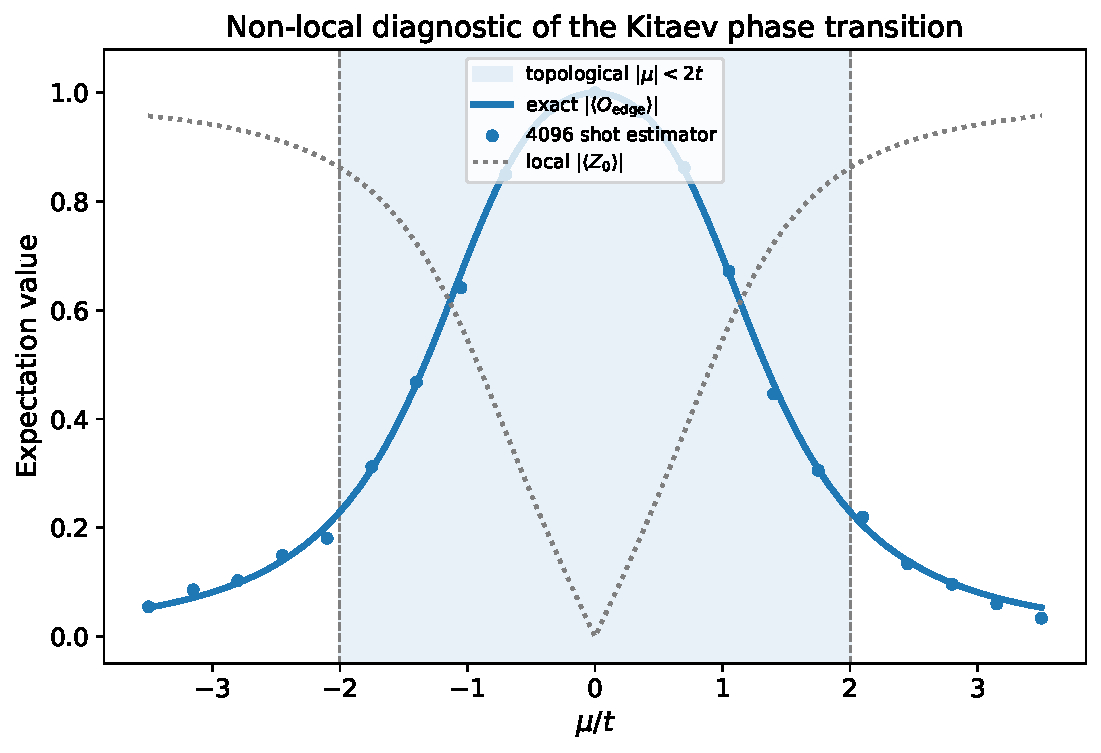
\includegraphics[width=0.95\linewidth]{../plots/block3_week6_phase_sweep.pdf}
  \caption{Week 6 phase sweep for $L=4$, $t=\Delta=1$. The left panel shows the non-local edge-string correlator and a finite-shot estimator. The right panel shows the parity-gap cross-check.}
\end{figure}

The shaded region marks the known topological interval
\begin{equation}
  |\mu|<2t.
\end{equation}
The expected qualitative behavior is:
\begin{itemize}
  \item inside the topological region, the two-edge string remains large because the boundary Majoranas are correlated through the non-local fermion;
  \item outside the topological region, the string drops because the chain becomes trivial and long-range edge correlation is lost;
  \item near $|\mu|=2t$, finite-size rounding replaces the sharp thermodynamic transition;
  \item the parity gap is small in the topological region and grows in the trivial region.
\end{itemize}

The left panel therefore gives the measurement-side signature, while the right panel gives a spectrum-side check from the qubit Hamiltonian. The point of the figure is not that exact diagonalization is the final algorithm. The point is that the chosen Pauli string carries the same phase information as the more traditional parity-gap diagnostic.
\section{Physical Interpretation of the Numerical Results}

The numerical sweep encodes three distinct regimes:

\subsection*{Topological phase ($|\mu| < 2t$)}
\begin{itemize}
  \item Majorana edge modes remain spatially separated.
  \item The non-local string remains finite.
  \item Edge-to-edge coherence is preserved.
\end{itemize}

\subsection*{Critical point ($|\mu| \approx 2t$)}
\begin{itemize}
  \item Bulk gap closes.
  \item Correlation length diverges.
  \item The system becomes highly sensitive to finite-size effects.
\end{itemize}

\subsection*{Trivial phase ($|\mu| > 2t$)}
\begin{itemize}
  \item Edge modes hybridize locally.
  \item Non-local correlations vanish.
  \item The string expectation collapses to zero.
\end{itemize}

This structure explains why the non-local correlator acts as a phase diagnostic.
\section{Connection to VQE}

The final Block 3 version should replace the exact even-parity eigenstate in the sweep with a VQE-prepared state
\begin{equation}
  \ket{\psi(\theta^*(\mu))}
  = U(\theta^*(\mu))\ket{0\cdots 0},
\end{equation}
where
\begin{equation}
  \theta^*(\mu) = \arg\min_{\theta}\ C_\mu(\theta).
\end{equation}
A parity-biased cost function can be reused from the Week 5 notebook:
\begin{equation}
  C_\mu(\theta)
  = \langle H(\mu)\rangle_\theta - \lambda\langle P\rangle_\theta,
  \qquad P=\prod_{j=0}^{L-1}Z_j.
\end{equation}
After optimization, the same Pauli-string measurement protocol estimates
\begin{equation}
  \langle\psi(\theta^*)|O_{\mathrm{edge}}|\psi(\theta^*)\rangle.
\end{equation}

The small-$L$ exact curve from Week 6 should be kept as a benchmark. It can answer whether VQE error, shot noise, or sign/string-convention mistakes are responsible when the circuit curve deviates from the expected phase diagram.
\section{Robustness Against Noise (Conceptual Outlook)}

Although Week 6 is formulated in an ideal setting, the observable is already structured for hardware implementation.

Expected effects of noise:
\begin{itemize}
  \item reduction of contrast in $\langle O_{\mathrm{edge}} \rangle$,
  \item smoothing of the phase boundary,
  \item but preservation of qualitative separation between phases for moderate noise.
\end{itemize}

This motivates Block 4, where depolarizing and readout noise models will be explicitly included in the circuit-level simulation.
\section{Bridge to Block 4}

Block 4 will ask whether this diagnostic survives realistic near-term hardware effects. The Week 6 curve defines the ideal reference. The natural Block 4 extensions are:
\begin{itemize}
  \item add depolarizing noise after one- and two-qubit gates;
  \item add readout error before classical bitstring processing;
  \item optionally add thermal relaxation through $T_1$ and $T_2$ parameters;
  \item compare ideal, noisy, and mitigated estimates of $|\langle O_{\mathrm{edge}}\rangle|$;
  \item quantify how much noise can be tolerated before the phase boundary is no longer visible.
\end{itemize}

In short, Week 6 finishes the ideal measurement story: a non-local Pauli string can be swept across $\mu$ and used as a circuit-compatible phase diagnostic. Block 4 will test the robustness of that diagnostic under noisy measurement and imperfect gates.

\end{document}
